Nous avons trouvé un contre exemple :
Soit G le graph défini comme suit : \newline
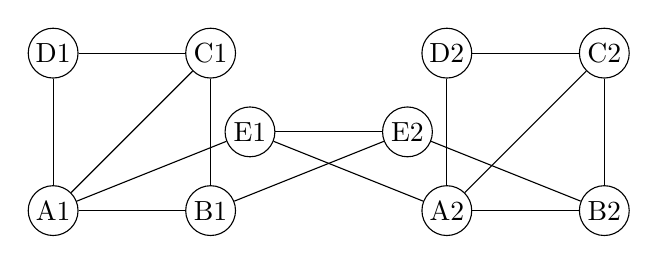
\begin{tikzpicture}[
  vertex/.style={circle, draw, minimum size=18pt, inner sep=0pt},
  scale=1
]

% --- G1: first square ---
\node[vertex] (A1) at (0,0) {A1};
\node[vertex] (B1) at (2,0) {B1};
\node[vertex] (C1) at (2,2) {C1};
\node[vertex] (D1) at (0,2) {D1};

% --- G1: second square ---
\node[vertex] (A2) at (5,0) {A2};
\node[vertex] (B2) at (7,0) {B2};
\node[vertex] (C2) at (7,2) {C2};
\node[vertex] (D2) at (5,2) {D2};

% --- Extra vertices ---
\node[vertex] (E1) at (2.5,1) {E1};
\node[vertex] (E2) at (4.5,1) {E2};

% --- Edges: first square ---
\draw (A1) -- (B1);
\draw (B1) -- (C1);
\draw (C1) -- (D1);
\draw (D1) -- (A1);
\draw (A1) -- (C1);

% --- Edges: second square ---
\draw (A2) -- (B2);
\draw (B2) -- (C2);
\draw (C2) -- (D2);
\draw (D2) -- (A2);
\draw (A2) -- (C2);

% --- Connecting edges ---
\draw (A1) -- (E1);
\draw (E1) -- (A2);
\draw (B1) -- (E2);
\draw (B2) -- (E2);
\draw (E1) -- (E2);

\end{tikzpicture}

On a que $k(G)$ la connexité minimale vaut 2.
Mais, si on applique la transformation $\psi$ sur l'arrète ${E_1, E_2}$
On obtient le graphe suivant : \newline

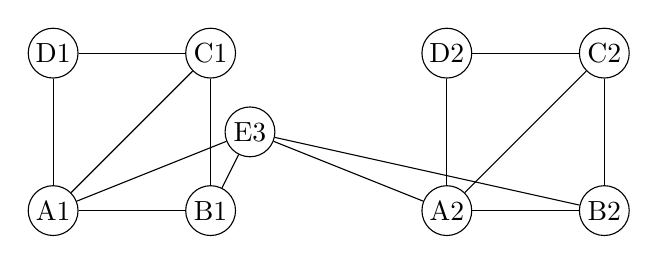
\begin{tikzpicture}[
  vertex/.style={circle, draw, minimum size=18pt, inner sep=0pt},
  scale=1
]

% --- G1: first square ---
\node[vertex] (A1) at (0,0) {A1};
\node[vertex] (B1) at (2,0) {B1};
\node[vertex] (C1) at (2,2) {C1};
\node[vertex] (D1) at (0,2) {D1};

% --- G1: second square ---
\node[vertex] (A2) at (5,0) {A2};
\node[vertex] (B2) at (7,0) {B2};
\node[vertex] (C2) at (7,2) {C2};
\node[vertex] (D2) at (5,2) {D2};

% --- Extra vertices ---
\node[vertex] (E3) at (2.5,1) {E3};

% --- Edges: first square ---
\draw (A1) -- (B1);
\draw (B1) -- (C1);
\draw (C1) -- (D1);
\draw (D1) -- (A1);
\draw (A1) -- (C1);

% --- Edges: second square ---
\draw (A2) -- (B2);
\draw (B2) -- (C2);
\draw (C2) -- (D2);
\draw (D2) -- (A2);
\draw (A2) -- (C2);

% --- Connecting edges ---
\draw (A1) -- (E3);
\draw (E3) -- (A2);
\draw (B1) -- (E3);
\draw (B2) -- (E3);

\end{tikzpicture}
\newline
Avec $k(\psi(G)) = 1$, donc $k(G) \ne k(\psi(G))$. Ainsi, $\psi$ ne conserve pas la connexité minimale.

